\documentclass{article}
\usepackage{array,graphicx,subcaption,float,booktabs,amsmath,amssymb,tikz,titlesec,indentfirst}
\usepackage{xeCJK}
\usepackage[letterpaper,top=1cm,bottom=2cm,left=2.5cm,right=2.5cm,marginparwidth=1.75cm]{geometry}
\def\degree{{}^{\circ}}
\setlength{\parindent}{2em}

\title{\huge{\textbf{CP第一次作业}}}
\author{黄羽翔 2100011536}
\date{\today}

\begin{document}
\large
\maketitle

\section{数值误差的避免}
\textbf{解题步骤:}设置变量存储每次计算结果,且统一使用double精度计算。停止条件为$|x_{k+1}-x_k|<\epsilon$,其中$\epsilon$为机器精度,即当$x_k=x_{k+1}$时停止迭代。\par

\renewcommand\arraystretch{1.2}
\begin{center}
\begin{tabular}{m{1.6cm}<{\centering}|m{3.2cm}<{\centering}|m{3.2cm}<{\centering}|m{3.2cm}<{\centering}|m{3.2cm}<{\centering}}
\hline
x取值&直接展开法&递归法&方法2计算$e^x$值&求倒数得$e^{-x}$值\\ \hline
0&1.0&1.0&1.0&1.0\\ 
10&4.53999294E-5&4.53999296E-5&2.20264657E+4&4.5399929E-5\\ 
20&6.13825973E-9&5.62188447E-9&4.85165195E+8&2.06115362E-9\\
30&-1.51730129E-4&-3.06681235E-5&1.06864745E+13&9.35762296E-14\\
40&3.74217741E+0&-3.16573189E+0&2.35385267E+0&4.24835426E-18\\
50&6.93150014E+4&1.10729334E+4&5.18470553E+21&1.92874985E-22\\
60&-1.13320491E+9&-3.35168107E+8&1.14200739E+26&8.75651076E-27\\
70&ERROR&-3.29796047E+13&2.51543867E+30&3.97544974E-31\\
80&ERROR&9.18056822E+16&5.54062238E+34&1.80485139E-35\\
90&ERROR&-5.05162535E+20&1.22040329E+39&8.19401262E-40\\
100&ERROR&-2.91375565E+24&2.68811714E+43&3.72007598E-44\\
\hline
\end{tabular}
\end{center}
\centerline{\textbf{Table 1:三种方法程序计算结果}}

\textbf{结果分析:}从表中可看出,直接展开法与递归法在前三项的计算结果在一定范围内相近,体现了算法的正确性。但在$x>=20$后,三种方法计算结果产生极大差异,而总有第三种方法最靠近真实值。\par
其原因在于,直接展开法与递归法在计算过程中,每次计算都会产生误差,并且在x较大的计算中,中间项存在远大于1的值,而最后计算结果过小,导致前两种算法由精度不足产生的误差此时会非常大。特别的,算法1产生的误差是来自于总计算结果,算法2产生的误差来自于每一项的计算结果,会导致算法1的误差大于算法2的误差,而二者差距会保持在一定范围(在表中可见算法1、2误差相差在x较大时保持在一个数量级左右)。而算法3尽管也存在同样的误差,但由于首先计算的是$e^{x}$的值,在求倒数后误差精度体现在有效位数的后面,因此误差相对较小。\par

\section{矩阵的模与条件数}
(a)\par
对于上三角矩阵(或下三角矩阵),其矩阵行列式值为对角项的乘积(代码有体现计算过程),又题目定义对角项均为1,故其行列式值为1。\par
(b)\par
利用高斯法,将A矩阵化为上三角矩阵:
$$
\begin{bmatrix}
    1 & -1 & ... & -1 & 1 & 0 & ... & 0\\
    0 & 1 & ... & -1 & 0 & 1 & ... & 0\\
    ... & ... & ... & ... & ... & ... & ... & ...\\
    0 & 0 & ... & 1 & 0 & 0 & ... & 1\\
\end{bmatrix}
$$
$$\downarrow \mathrm{Gauss}$$
$$
\begin{bmatrix}
    1 & 0 & ... & 0 & 1 & 1 & ... & 2^{n-2}\\
    0 & 1 & ... & 0 & 0 & 1 & ... & 2^{n-3}\\
    ... & ... & ... & ... & ... & ... & ... & ...\\
    0 & 0 & ... & 1 & 0 & 0 & ... & 1\\
\end{bmatrix}
$$
\par
则$\mathrm{A}^{-1}$为:
$$
A^{-1}=
\begin{bmatrix}
    1 & 1 & ... & n-1\\
    0 & 1 & ... & n-2\\
    ... & ... & ... & ...\\
    0 & 0 & ... & 1\\
\end{bmatrix}
$$
\par
(c)\par
若采用矩阵p模的定义(以及矢量p模的定义),则对于$\infty$模,有:
$$||\vec x||_\infty=\left(\sum_{i=1}^n|x_i|^\infty\right)^{\frac{1}{\infty}}=\max_{1\leq i\leq n}|x_i|$$
$$||A||_\infty=\sup_{\vec x\neq 0}\frac{||A\vec x||_\infty}{||\vec x||_\infty}=\sup_{\vec x\neq 0}\frac{||A\vec x||_\infty}{\max_{1\leq i\leq n}|x_i|}$$
\par
设
$$\vec y=A \vec x$$
\par 
则
$$||\vec y||_\infty=\max_{1\leq i\leq n}|y_i|=\max_{1\leq i\leq n}\left|\sum_{j=1}^n a_{ij}x_j\right|$$
\par
若满足条件的项分别为$y_{i1},x_{i2}$,若$i1\neq i2$,则$x_{i1}<x_{i2}$,有
$$\frac{||\vec y||}{||\vec x||}=|\frac{y_{i1}}{x_{i2}}|\leq \max_{1\leq i\leq n}\sum_{j=1}^n|a_{ij}|$$
\par
当且仅当$i1=i2$时,不等式取等,此时满足$\sup$条件,即
$$||A||_\infty=|\frac{y_{i1}}{x_{i1}}|=\max_{1\leq i\leq n}\sum_{j=1}^n|a_{ij}|$$
\par
(d)\par
对于p=2的欧式模,幺正矩阵$U$有:
$$||U||_2=\sup_{\vec x\neq 0}\frac{||U\vec x||_2}{||\vec x||_2}=\sup_{\vec x\neq 0}\frac{||U\vec x||_2}{|\vec x|^2}$$
\par
由定义
$$||U\vec x||_2=\sqrt{\sum_{i=1}^n\left(\sum_{j=1}^n u_{ij}x_j\right)^2}=\sqrt{x^\dag U^\dag Ux}=\sqrt{x^\dag x}=||\vec x||_2=|\vec x|^2$$
\par
则有
$$||U||_2=\sup_{\vec x\neq 0}\frac{|\vec x|^2}{|\vec x|^2}=1$$
\par
将全体$U$替换为$U^\dag$,所有$U^\dag$替换为$U$,则完成另一个证明\par
类似的,对于$||UA||_2$有
$$||UA||_2=\sup_{x\neq 0}\frac{||UA\vec x||_2}{||\vec x||_2}=\sup_{x\neq 0}\frac{||UA\vec x||_2}{|\vec x|^2}$$
\par
而
$$||UA\vec x||_2=\sqrt{\sum_{i=1}^n\left(\sum_{j=1}^n u_{ij}a_{jk}x_k\right)^2}=\sqrt{x^\dag A^\dag U^\dag UAx}=\sqrt{x^\dag A^\dag A x}=||A\vec x||_2$$
\par
则
$$||UA||_2=\sup_{x\neq 0}\frac{||A\vec x||_2}{|\vec x|^2}=||A||_2$$
\par
如果利用欧氏模来定义条件数,则
$$K_2(A)=||A||_2||A^{-1}||_2=||UA||_2||U^\dag A^{-1}||_2=K_2(UA)$$
\par
(e)\par
对于上述$A$定义,结合前文所求,有
$$||A||_\infty=\max_{1\leq i\leq n}\sum_{j=1}^n|a_{ij}|=\sum_{i=1,j}|a_{ij}|=n$$
$$||A^{-1}||_\infty=\max_{1\leq i\leq n}\sum_{j=1}^n|a_{ij}|=\sum_{i=1,j}|a_{ij}|=2^{n-1}$$
$$K_\infty(A)=||A||_\infty||A^{-1}||_\infty=n\times 2^{n-1}$$

\section{Hilbert矩阵}

(a)\par
若满足
$$D=D_{\min}=\int_0^1\left(\sum_{i=1}^nc_ix^{i-1}-f(x)\right)^2\mathrm{d}x$$
\par
则有
$$\delta \left(\int_0^1\left(\sum_{i=1}^nc_ix^{i-1}-f(x)\right)^2\mathrm{d}x\right)=\delta D=0$$
\par
又
\begin{equation}
    \begin{gathered}
     \begin{split}
        \delta D=&\delta \left(\int_0^1\left(\sum_{i=1}^nc_ix^{i-1}-f(x)\right)^2\mathrm{d}x\right)\\
        =&\int_0^1\delta\left(\left(\sum_{i=1}^nc_ix^{i-1}-f(x)\right)^2\right)\mathrm{d}x\\
        =&\int_0^1d\mathrm{x}\left(\frac{\partial}{\partial c_1}\left(\sum_{i=1}^nc_ix^{i-1}-f(x)\right)^2\delta c_1+...\frac{\partial}{\partial c_n}\left(\sum_{i=1}^nc_ix^{i-1}-f(x)\right)^2\delta c_n\right)\\
        =&\int_0^1\left(2\left(\sum_{i=1}^nc_ix^{i-1}-f(x)\right)\left(\sum_{j=1}^n\delta c_jx^{j-1}\right)\right)\mathrm{d}x\\
        =&2\sum_{j=1}^n\delta c_j\left(\sum_{i=1}^n\frac{1}{i+j-1}c_i-\int_0^1f(x)x^{j-1}\mathrm{d}x\right)=0
    \notag
    \end{split}
    \end{gathered}
\end{equation}
\par
对每一个$\delta c_j$均满足约束,则满足约束矩阵方程
$$
H\vec c=\vec b
$$
\par
其中$H_{ij}=\frac{1}{i+j-1}$为Hilbert矩阵,$\vec c=\{c_1,...,c_n\}^T$为待求系数向量,$\vec b=\{\int_0^1f(x)x^0\mathrm{d}x,...,\int_0^1f(x)x^{n-1}\mathrm{d}x\}$为约束向量
\par
(b)\par
利用数学归纳法,对于$n=1$,显然成立。假设对于$n=k$成立,即
$$
|H_n|=
\left|
\begin{matrix}
    1 & \frac{1}{2} & ... & \frac{1}{k}\\
    \frac{1}{2} & \frac{1}{3} & ... & \frac{1}{k+1}\\
    ... & ... & ... & ...\\
    \frac{1}{k} & \frac{1}{k+1} & ... & \frac{1}{2k-1}\\
\end{matrix}
\right|
>0
$$
则对于$n=k+1$,有
\begin{equation}
    \begin{gathered}
     \begin{split}
|H_{k+1,0}|&=
\left|
\begin{matrix}
    1 & \frac{1}{2} & ... & \frac{1}{k} & \frac{1}{k+1}\\
    \frac{1}{2} & \frac{1}{3} & ... & \frac{1}{k+1} & \frac{1}{k+2}\\
    ... & ... & ... & ... & ...\\
    \frac{1}{k} & \frac{1}{k+1} & ... & \frac{1}{2k-1} & \frac{1}{2k}\\
    \frac{1}{k+1} & \frac{1}{k+2} & ... & \frac{1}{2k} & \frac{1}{2k+1}\\
\end{matrix}
\right|\\
&=\left|
\begin{matrix}
    1 & \frac{1}{2} & ... & \frac{1}{k} & \frac{1}{k+1}\\
    \frac{1}{2}-\frac{1}{2} & \frac{1}{3}-\frac{1}{2}\times \frac{1}{2} & ... & \frac{1}{k+1}-\frac{1}{2}\times \frac{1}{k} & \frac{1}{k+2}-\frac{1}{2}\times \frac{1}{k+1}\\
    ... & ... & ... & ... & ...\\
    \frac{1}{k}-\frac{1}{k} & \frac{1}{k+1}-\frac{1}{k}\times \frac{1}{2} & ... & \frac{1}{2k-1}-\frac{1}{k}\times \frac{1}{k} & \frac{1}{2k}-\frac{1}{k}\times \frac{1}{k+1}\\
    \frac{1}{k+1}-\frac{1}{k+1} & \frac{1}{k+2}-\frac{1}{k+1}\times \frac{1}{2} & ... & \frac{1}{2k}-\frac{1}{k+1}\times \frac{1}{k} & \frac{1}{2k+1}-\frac{1}{k+1}\times \frac{1}{k+1}\\
\end{matrix}
\right|\\
&=\left|
\begin{matrix}
    1 & \frac{1}{2} & ... & \frac{1}{k} & \frac{1}{k+1}\\
    0 & \frac{1}{12} & ... & \frac{k-1}{2k(k+1)} & \frac{k}{2(k+1)(k+2)}\\
    ... & ... & ... & ... & ...\\
    0 & \frac{k-1}{2k(k+1)} & ... & \frac{k^2-2k+1}{k^2(2k-1)} & \frac{k^2-k}{2k^2(k+1)}\\
    0 & \frac{k}{2(k+1)(k+2)} & ... & \frac{k^2-k}{2k^2(2k+1)} & \frac{k^2}{(k+1)^2(2k+3)}\\
\end{matrix}
\right|\\
&=\left|
\begin{matrix}
    \frac{1}{12} & ... & \frac{k-1}{2k(k+1)} & \frac{k}{2(k+1)(k+2)}\\
    ... & ... & ... & ...\\
    \frac{k-1}{2k(k+1)} & ... & \frac{k^2-2k+1}{k^2(2k-1)} & \frac{k^2-k}{2k^2(k+1)}\\
    \frac{k}{2(k+1)(k+2)} & ... & \frac{k^2-k}{2k^2(2k+1)} & \frac{k^2}{(k+1)^2(2k+3)}\\
\end{matrix}
\right|\\
&=(k!)^2\frac{1}{2^2\times3^2\times...\times (k+1)^2} H_{k+1,2}\\
&\neq 0
\notag
\end{split}
\end{gathered}
\end{equation}
\par
即证明$H_n$正定,而其行列式不为0也显然说明$H_n$是非奇异的\par
(c)\par
计算结果见代码\par
可以发现$H_n$以$2^{-n^2}$的量级多级指数衰减
\par 
(d)\par
具体计算结果见代码,结果如下图所示:(实在懒得打表hh)
\begin{figure}[H]
    \centering
    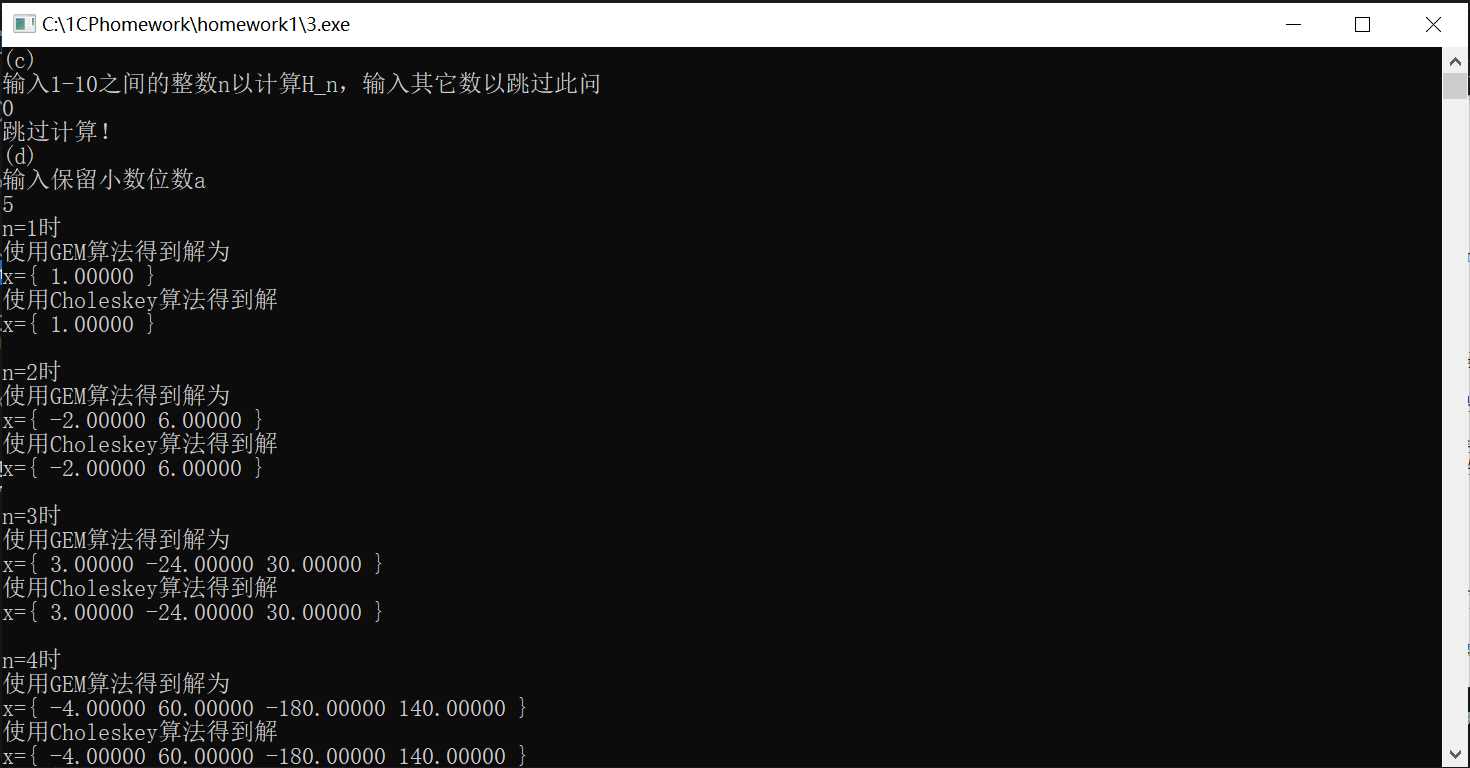
\includegraphics[width=12cm]{1.png}
    \caption{}
\end{figure}
\begin{figure}[H]
    \centering
    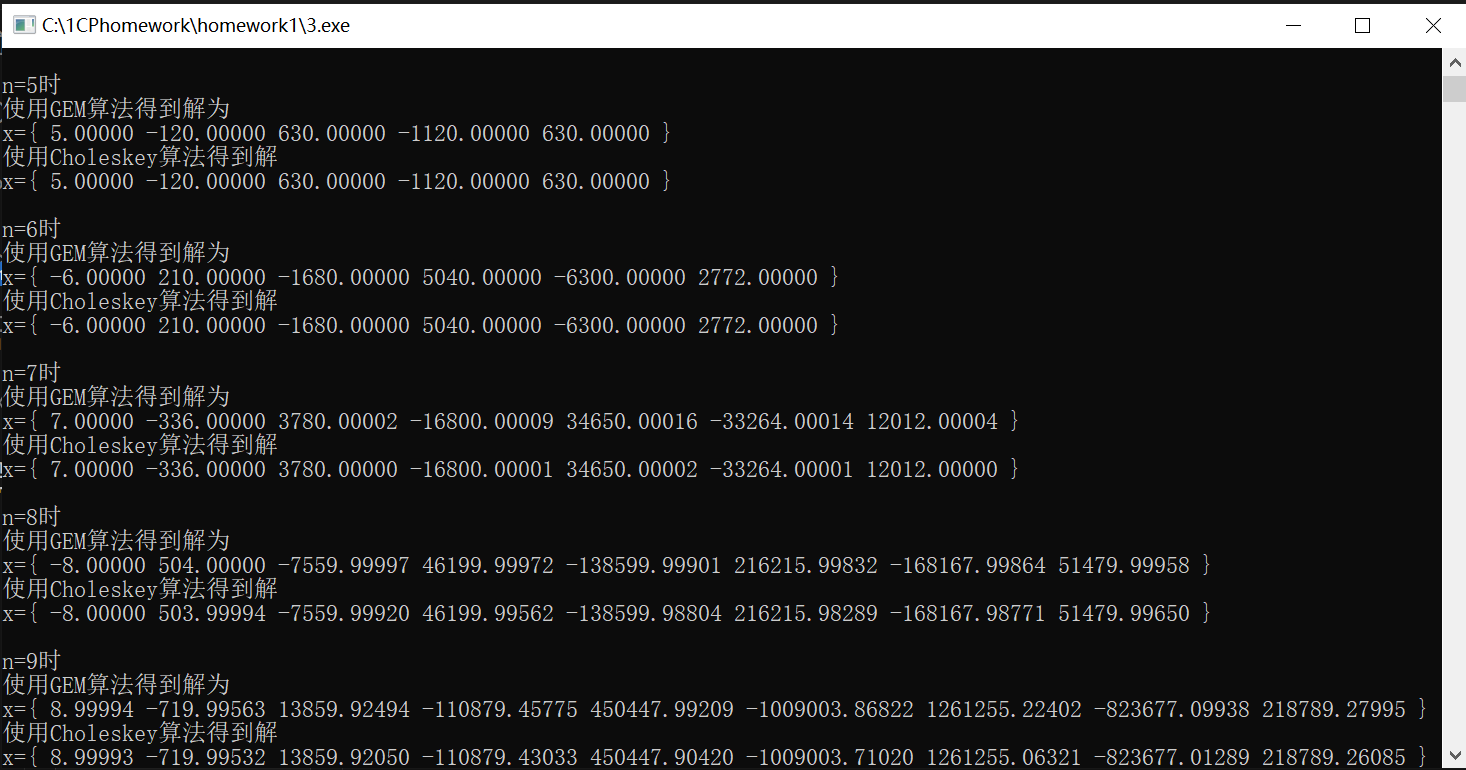
\includegraphics[width=12cm]{2.png}
    \caption{}
\end{figure}
可看出两种解法结果在n较大时有微小的差别。由于Choleskey分解具有高稳定性,其计算精度应当更高。

\section{矩阵与二次型}
\par
(a)\par
满足
$$|\lambda I-B|=0$$
$$(\lambda I-B)\vec x=\vec 0$$
化为
$$(\lambda-1)(\lambda-2)(\lambda-1)+(1-\lambda)\times 1\times 1+(1-\lambda)\times 1\times 1=0$$
$$\lambda^3-4\lambda^2+3\lambda=0$$
$$\lambda(\lambda-1)(\lambda-3)=0$$
特征值为
$$\lambda_1=0,\lambda_2=1,\lambda_3=3$$
对应特征向量为
$$\vec x_1=\{\frac{\sqrt 3}{3},\frac{\sqrt 3}{3},\frac{\sqrt 3}{3}\}$$
$$\vec x_2=\{\frac{\sqrt 2}{2},0,-\frac{\sqrt 2}{2}\}$$
$$\vec x_3=\{\frac{\sqrt 6}{6},-\frac{2\sqrt 6}{6},\frac{\sqrt 6}{6}\}$$
\par
(b)\par
$Q$为$\vec x$的组合,满足
$$Q=\left[\vec x_1^T,\vec x_2^T,\vec x_3^T\right]=
\begin{bmatrix}
    \frac{\sqrt 3}{3} & \frac{\sqrt 2}{2} & \frac{\sqrt 6}{6}\\
    \frac{\sqrt 3}{3} & 0 & -\frac{2\sqrt 6}{6}\\
    \frac{\sqrt 3}{3} & -\frac{\sqrt 2}{2} & \frac{\sqrt 6}{6}\\   
\end{bmatrix}
$$
$$
Q^{-1}=Q^T=
\begin{bmatrix}
    \frac{\sqrt 3}{3} & \frac{\sqrt 3}{3} & \frac{\sqrt 3}{3}\\
    \frac{\sqrt 2}{2} & 0 & -\frac{\sqrt 2}{2}\\
    \frac{\sqrt 6}{6} & -\frac{2\sqrt 6}{6} & \frac{\sqrt 6}{6}\\
\end{bmatrix}
$$
$$
\Sigma=
\begin{bmatrix}
    \lambda_1 & 0 & 0\\
    0 & \lambda_2 & 0\\
    0 & 0 & \lambda_3\\
\end{bmatrix}
=
\begin{bmatrix}
    0 & 0 & 0\\
    0 & 1 & 0\\
    0 & 0 & 3\\
\end{bmatrix}
$$
\par
设
$$\vec u=\{x,y,z\}^T$$
则有
$$\vec u^T B\vec u=x^2+2y^2+z^2-2xy-yz=(x-y)^2+1/2(y-z)^2+1/2y^2+1/2z^2=2$$
利用mathematica绘图
\begin{figure}[H]
    \centering
    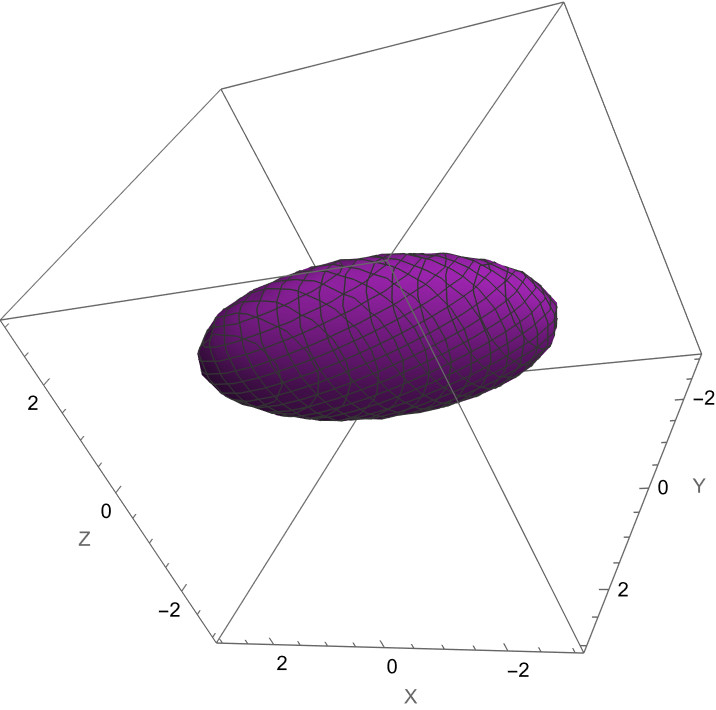
\includegraphics[width=11cm]{mathematica1.png}
    \caption{}
\end{figure}
类似的,三个特征向量图像为
\begin{figure}[H]
    \centering
    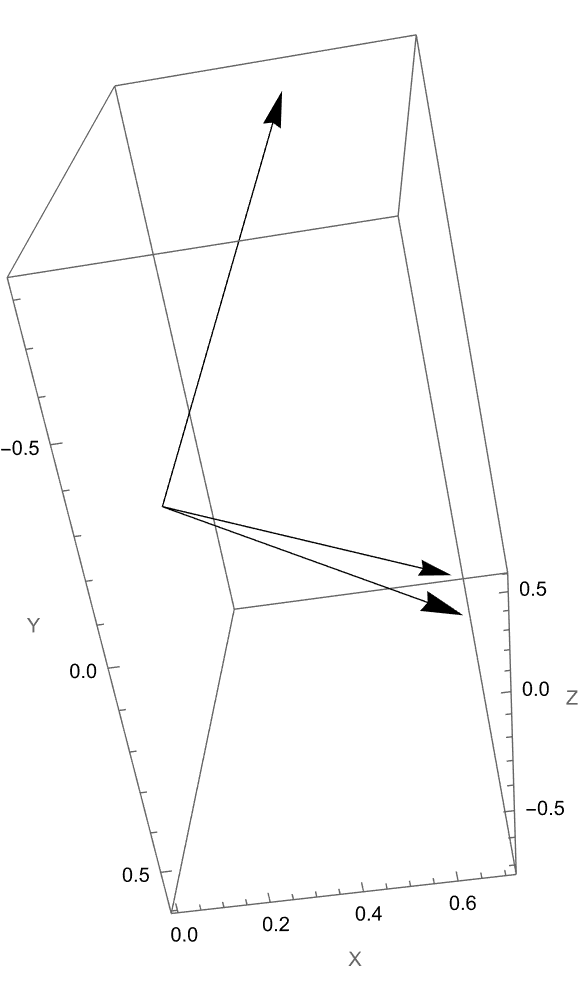
\includegraphics[width=10cm]{mathematica2.png}
    \caption{}
\end{figure}
绘图mathematica代码附在文件中

\section{正定矩阵}
\par
(a)\par
对于$\vec u=\{x_1,x_2,x_3,x_4\}^T$,有
$$\vec u^TA^T=\{x_1,x_2-x_1,x_3-x_2, x_4-x_3,-x_4\}^T$$
\par
则
$$\vec u^TA^TA\vec u=x_1^2+(x_2-x_1)^2+(x_3-x_2)^2+(x_4-x_3)^2+x_4^2\geq 0$$
\par
很明显,对于能分解为$A^TA$形式的矩阵,均有
$$\vec u^TA^TA\vec u=\sum_i \left(\sum_j a_{ij}u_j\right)^2\geq 0$$
\par
又对于本式,取等条件为
\begin{equation}
    \begin{gathered}
     \left\{
     \begin{split}
        &x_1=0\\
        &x_2=x_1\\
        &x_3=x_2\\
        &x_4=x_3\\
        &x_4=0
        \notag
     \end{split}
    \right.
    \end{gathered}
\end{equation}
\par
当且仅当
$$\vec u=\{0,0,0,0\}^T$$
\par
时成立,故$\vec u\neq 0$时,$\vec u^TA^TA\vec u>0$,得证\par
(b)\par
设$\vec u=\{x,y\}$,有:
$$\vec u^TS\vec u=2x^2+bxy+bxy+4y^2$$
\begin{equation}
    \begin{gathered}
     \begin{split}
        \vec u^TS\vec u&=2x^2+bxy+bxy+4y^2\\
        &=2(x+\sqrt 2y)^2+(2b-4\sqrt 2)xy
        \notag
     \end{split}
    \end{gathered}
\end{equation}
\par
当$-2\sqrt 2<b<2\sqrt 2$时,原式可配为完全平方和
$$\vec u^TS\vec u=\frac{b}{\sqrt 2}(x+\sqrt 2y)^2+(2-b/\sqrt 2)x^2+2(2-b/\sqrt 2)y^2> 0$$
\par
此时原矩阵为正定
\par
当$b=\pm 2\sqrt 2$时,原式恰可配为完全平方和
$$\vec u^TS\vec u=2(x\pm \sqrt 2y)^2\geq 0$$
\par
此时原矩阵为半正定
\par
当$b>2\sqrt 2$时,原式不可配为完全平方和,故不是正定矩阵

\end{document}



\renewcommand\arraystretch{1.2}
\begin{center}
\begin{tabular}{|m{2cm}<{\centering}|}
\hline
内容\\ \hline
\end{tabular}
\end{center}
\centerline{\textbf{Table 1:注释}}

\begin{figure}[H]
    \centering
    \includegraphics[width=12cm]{}
    \caption{}
\end{figure}

\begin{equation}
    \begin{gathered}
     \left\{
     \begin{split}
     \end{split}
    \right.
    \end{gathered}
\end{equation}
 
 \begin{figure}[H]
\centering
\begin{minipage}[t]{0.48\textwidth}
\centering
\includegraphics[width=7cm]{图片1}
\caption{}
\end{minipage}
\begin{minipage}[t]{0.48\textwidth}
\centering
\includegraphics[width=7cm]{图片2}
\caption{}
\end{minipage}
\end{figure}